\documentclass[1p]{elsarticle_modified}
%\bibliographystyle{elsarticle-num}

%\usepackage[colorlinks]{hyperref}
%\usepackage{abbrmath_seonhwa} %\Abb, \Ascr, \Acal ,\Abf, \Afrak
\usepackage{amsfonts}
\usepackage{amssymb}
\usepackage{amsmath}
\usepackage{amsthm}
\usepackage{scalefnt}
\usepackage{amsbsy}
\usepackage{kotex}
\usepackage{caption}
\usepackage{subfig}
\usepackage{color}
\usepackage{graphicx}
\usepackage{xcolor} %% white, black, red, green, blue, cyan, magenta, yellow
\usepackage{float}
\usepackage{setspace}
\usepackage{hyperref}

\usepackage{tikz}
\usetikzlibrary{arrows}

\usepackage{multirow}
\usepackage{array} % fixed length table
\usepackage{hhline}

%%%%%%%%%%%%%%%%%%%%%
\makeatletter
\renewcommand*\env@matrix[1][\arraystretch]{%
	\edef\arraystretch{#1}%
	\hskip -\arraycolsep
	\let\@ifnextchar\new@ifnextchar
	\array{*\c@MaxMatrixCols c}}
\makeatother %https://tex.stackexchange.com/questions/14071/how-can-i-increase-the-line-spacing-in-a-matrix
%%%%%%%%%%%%%%%

\usepackage[normalem]{ulem}

\newcommand{\msout}[1]{\ifmmode\text{\sout{\ensuremath{#1}}}\else\sout{#1}\fi}
%SOURCE: \msout is \stkout macro in https://tex.stackexchange.com/questions/20609/strikeout-in-math-mode

\newcommand{\cancel}[1]{
	\ifmmode
	{\color{red}\msout{#1}}
	\else
	{\color{red}\sout{#1}}
	\fi
}

\newcommand{\add}[1]{
	{\color{blue}\uwave{#1}}
}

\newcommand{\replace}[2]{
	\ifmmode
	{\color{red}\msout{#1}}{\color{blue}\uwave{#2}}
	\else
	{\color{red}\sout{#1}}{\color{blue}\uwave{#2}}
	\fi
}

\newcommand{\Sol}{\mathcal{S}} %segment
\newcommand{\D}{D} %diagram
\newcommand{\A}{\mathcal{A}} %arc


%%%%%%%%%%%%%%%%%%%%%%%%%%%%%5 test

\def\sl{\operatorname{\textup{SL}}(2,\Cbb)}
\def\psl{\operatorname{\textup{PSL}}(2,\Cbb)}
\def\quan{\mkern 1mu \triangleright \mkern 1mu}

\theoremstyle{definition}
\newtheorem{thm}{Theorem}[section]
\newtheorem{prop}[thm]{Proposition}
\newtheorem{lem}[thm]{Lemma}
\newtheorem{ques}[thm]{Question}
\newtheorem{cor}[thm]{Corollary}
\newtheorem{defn}[thm]{Definition}
\newtheorem{exam}[thm]{Example}
\newtheorem{rmk}[thm]{Remark}
\newtheorem{alg}[thm]{Algorithm}

\newcommand{\I}{\sqrt{-1}}
\begin{document}

%\begin{frontmatter}
%
%\title{Boundary parabolic representations of knots up to 8 crossings}
%
%%% Group authors per affiliation:
%\author{Yunhi Cho} 
%\address{Department of Mathematics, University of Seoul, Seoul, Korea}
%\ead{yhcho@uos.ac.kr}
%
%
%\author{Seonhwa Kim} %\fnref{s_kim}}
%\address{Center for Geometry and Physics, Institute for Basic Science, Pohang, 37673, Korea}
%\ead{ryeona17@ibs.re.kr}
%
%\author{Hyuk Kim}
%\address{Department of Mathematical Sciences, Seoul National University, Seoul 08826, Korea}
%\ead{hyukkim@snu.ac.kr}
%
%\author{Seokbeom Yoon}
%\address{Department of Mathematical Sciences, Seoul National University, Seoul, 08826,  Korea}
%\ead{sbyoon15@snu.ac.kr}
%
%\begin{abstract}
%We find all boundary parabolic representation of knots up to 8 crossings.
%
%\end{abstract}
%\begin{keyword}
%    \MSC[2010] 57M25 
%\end{keyword}
%
%\end{frontmatter}

%\linenumbers
%\tableofcontents
%
\newcommand\colored[1]{\textcolor{white}{\rule[-0.35ex]{0.8em}{1.4ex}}\kern-0.8em\color{red} #1}%
%\newcommand\colored[1]{\textcolor{white}{ #1}\kern-2.17ex	\textcolor{white}{ #1}\kern-1.81ex	\textcolor{white}{ #1}\kern-2.15ex\color{red}#1	}

{\Large $\underline{11n_{84}~(K11n_{84})}$}

\setlength{\tabcolsep}{10pt}
\renewcommand{\arraystretch}{1.6}
\vspace{1cm}\begin{tabular}{m{100pt}>{\centering\arraybackslash}m{274pt}}
\multirow{5}{120pt}{
	\centering
	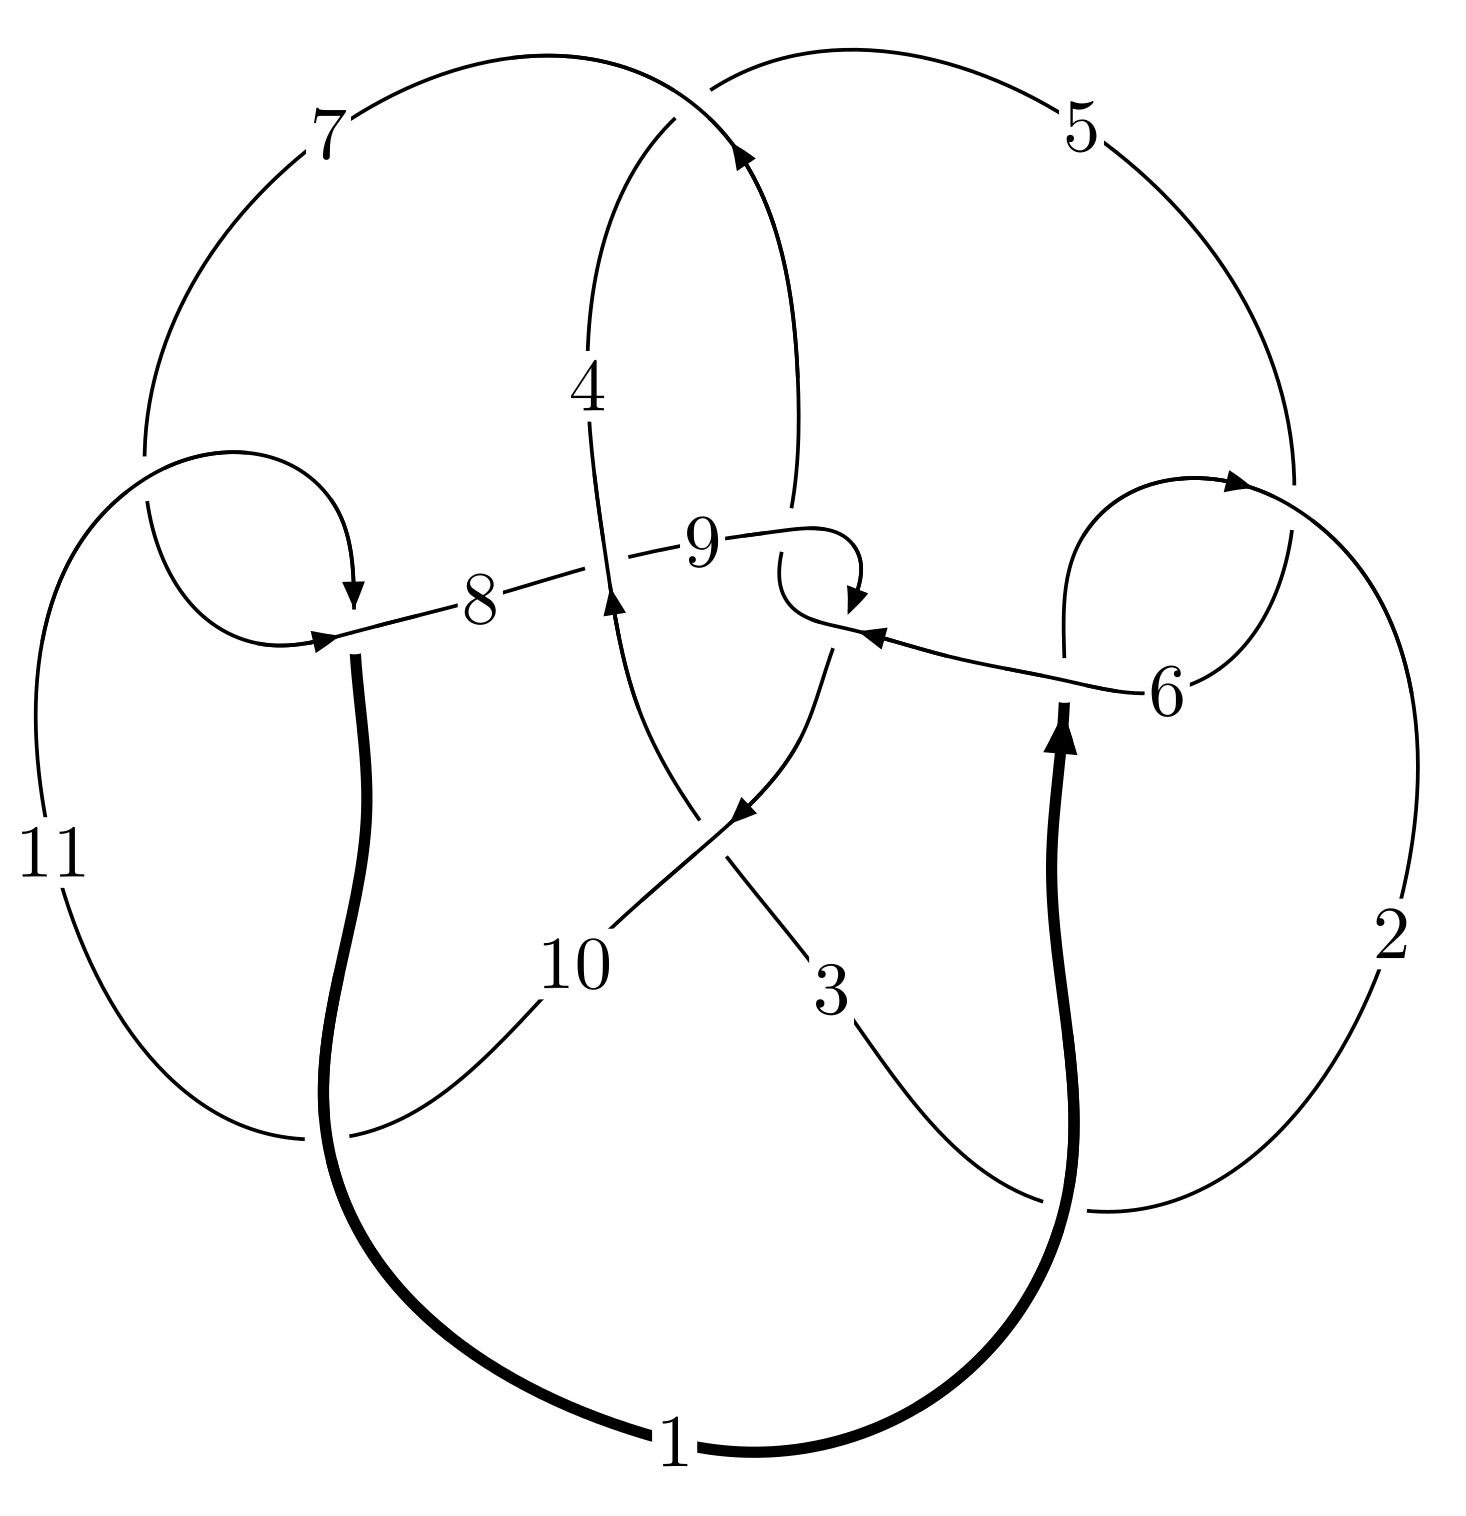
\includegraphics[width=112pt]{../../../GIT/diagram.site/Diagrams/png/700_11n_84.png}\\
\ \ \ A knot diagram\footnotemark}&
\allowdisplaybreaks
\textbf{Linearized knot diagam} \\
\cline{2-2}
 &
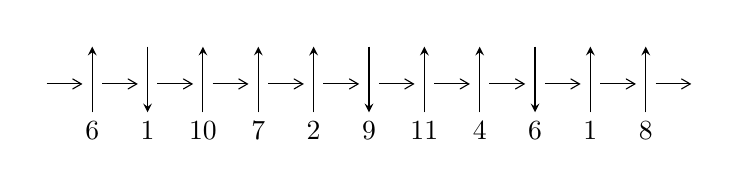
\begin{tikzpicture}[x=20pt, y=17pt]
	% nodes
	\node (C0) at (0, 0) {};
	\node (C1) at (1, 0) {};
	\node (C1U) at (1, +1) {};
	\node (C1D) at (1, -1) {6};

	\node (C2) at (2, 0) {};
	\node (C2U) at (2, +1) {};
	\node (C2D) at (2, -1) {1};

	\node (C3) at (3, 0) {};
	\node (C3U) at (3, +1) {};
	\node (C3D) at (3, -1) {10};

	\node (C4) at (4, 0) {};
	\node (C4U) at (4, +1) {};
	\node (C4D) at (4, -1) {7};

	\node (C5) at (5, 0) {};
	\node (C5U) at (5, +1) {};
	\node (C5D) at (5, -1) {2};

	\node (C6) at (6, 0) {};
	\node (C6U) at (6, +1) {};
	\node (C6D) at (6, -1) {9};

	\node (C7) at (7, 0) {};
	\node (C7U) at (7, +1) {};
	\node (C7D) at (7, -1) {11};

	\node (C8) at (8, 0) {};
	\node (C8U) at (8, +1) {};
	\node (C8D) at (8, -1) {4};

	\node (C9) at (9, 0) {};
	\node (C9U) at (9, +1) {};
	\node (C9D) at (9, -1) {6};

	\node (C10) at (10, 0) {};
	\node (C10U) at (10, +1) {};
	\node (C10D) at (10, -1) {1};

	\node (C11) at (11, 0) {};
	\node (C11U) at (11, +1) {};
	\node (C11D) at (11, -1) {8};
	\node (C12) at (12, 0) {};

	% arrows
	\draw[->,>={angle 60}]
	(C0) edge (C1) (C1) edge (C2) (C2) edge (C3) (C3) edge (C4) (C4) edge (C5) (C5) edge (C6) (C6) edge (C7) (C7) edge (C8) (C8) edge (C9) (C9) edge (C10) (C10) edge (C11) (C11) edge (C12) ;	\draw[->,>=stealth]
	(C1D) edge (C1U) (C2U) edge (C2D) (C3D) edge (C3U) (C4D) edge (C4U) (C5D) edge (C5U) (C6U) edge (C6D) (C7D) edge (C7U) (C8D) edge (C8U) (C9U) edge (C9D) (C10D) edge (C10U) (C11D) edge (C11U) ;
	\end{tikzpicture} \\
\hhline{~~} \\& 
\textbf{Solving Sequence} \\ \cline{2-2} 
 &
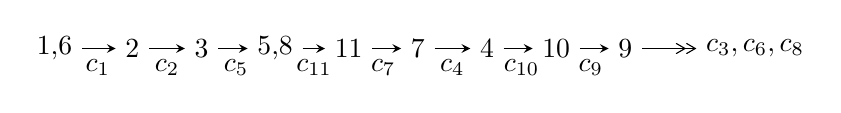
\begin{tikzpicture}[x=25pt, y=7pt]
	% node
	\node (A0) at (-1/8, 0) {1,6};
	\node (A1) at (1, 0) {2};
	\node (A2) at (2, 0) {3};
	\node (A3) at (49/16, 0) {5,8};
	\node (A4) at (33/8, 0) {11};
	\node (A5) at (41/8, 0) {7};
	\node (A6) at (49/8, 0) {4};
	\node (A7) at (57/8, 0) {10};
	\node (A8) at (65/8, 0) {9};
	\node (C1) at (1/2, -1) {$c_{1}$};
	\node (C2) at (3/2, -1) {$c_{2}$};
	\node (C3) at (5/2, -1) {$c_{5}$};
	\node (C4) at (29/8, -1) {$c_{11}$};
	\node (C5) at (37/8, -1) {$c_{7}$};
	\node (C6) at (45/8, -1) {$c_{4}$};
	\node (C7) at (53/8, -1) {$c_{10}$};
	\node (C8) at (61/8, -1) {$c_{9}$};
	\node (A9) at (10, 0) {$c_{3},c_{6},c_{8}$};

	% edge
	\draw[->,>=stealth]	
	(A0) edge (A1) (A1) edge (A2) (A2) edge (A3) (A3) edge (A4) (A4) edge (A5) (A5) edge (A6) (A6) edge (A7) (A7) edge (A8) ;
	\draw[->>,>={angle 60}]	
	(A8) edge (A9);
\end{tikzpicture} \\ 

\end{tabular} \\

\footnotetext{
The image of knot diagram is generated by the software ``\textbf{Draw programme}" developed by Andrew Bartholomew(\url{http://www.layer8.co.uk/maths/draw/index.htm\#Running-draw}), where we modified some parts for our purpose(\url{https://github.com/CATsTAILs/LinksPainter}).
}\phantom \\ \newline 
\centering \textbf{Ideals for irreducible components\footnotemark of $X_{\text{par}}$} 
 
\begin{align*}
I^u_{1}&=\langle 
3 u^8+4 u^7+24 u^6+25 u^5+51 u^4+41 u^3+6 u^2+4 b+3 u+5,\\
\phantom{I^u_{1}}&\phantom{= \langle  }- u^8-2 u^7-8 u^6-13 u^5-17 u^4-21 u^3+4 a+5 u+3,\\
\phantom{I^u_{1}}&\phantom{= \langle  }u^9+2 u^8+9 u^7+14 u^6+24 u^5+27 u^4+15 u^3+5 u^2+3 u+1\rangle \\
I^u_{2}&=\langle 
-347 u^{13}-980 u^{12}+\cdots+877 b-863,\;-2540 u^{13}-9801 u^{12}+\cdots+877 a-12943,\\
\phantom{I^u_{2}}&\phantom{= \langle  }u^{14}+4 u^{13}+\cdots+19 u+1\rangle \\
I^u_{3}&=\langle 
- a u+b- a- u-1,\;a^2+2 a+2,\;u^2+u+1\rangle \\
I^u_{4}&=\langle 
b- u,\;a- u+1,\;u^2- u+1\rangle \\
I^u_{5}&=\langle 
a u+b- u-1,\;a^2+2 a u- u,\;u^2+u+1\rangle \\
\\
\end{align*}
\raggedright * 5 irreducible components of $\dim_{\mathbb{C}}=0$, with total 33 representations.\\
\footnotetext{All coefficients of polynomials are rational numbers. But the coefficients are sometimes approximated in decimal forms when there is not enough margin.}
\newpage
\renewcommand{\arraystretch}{1}
\centering \section*{I. $I^u_{1}= \langle 3 u^8+4 u^7+\cdots+4 b+5,\;- u^8-2 u^7+\cdots+4 a+3,\;u^9+2 u^8+\cdots+3 u+1 \rangle$}
\flushleft \textbf{(i) Arc colorings}\\
\begin{tabular}{m{7pt} m{180pt} m{7pt} m{180pt} }
\flushright $a_{1}=$&$\begin{pmatrix}1\\0\end{pmatrix}$ \\
\flushright $a_{6}=$&$\begin{pmatrix}0\\u\end{pmatrix}$ \\
\flushright $a_{2}=$&$\begin{pmatrix}1\\- u^2\end{pmatrix}$ \\
\flushright $a_{3}=$&$\begin{pmatrix}u^2+1\\- u^2\end{pmatrix}$ \\
\flushright $a_{5}=$&$\begin{pmatrix}- u\\u^3+u\end{pmatrix}$ \\
\flushright $a_{8}=$&$\begin{pmatrix}\frac{1}{4} u^8+\frac{1}{2} u^7+\cdots-\frac{5}{4} u-\frac{3}{4}\\-\frac{3}{4} u^8- u^7+\cdots-\frac{3}{4} u-\frac{5}{4}\end{pmatrix}$ \\
\flushright $a_{11}=$&$\begin{pmatrix}\frac{1}{4} u^8+\frac{1}{4} u^7+\cdots+\frac{1}{4} u+2\\- u\end{pmatrix}$ \\
\flushright $a_{7}=$&$\begin{pmatrix}u^8+\frac{5}{4} u^7+\cdots-2 u+\frac{1}{4}\\-\frac{1}{4} u^8-\frac{1}{4} u^7+\cdots+\frac{1}{4} u-\frac{1}{2}\end{pmatrix}$ \\
\flushright $a_{4}=$&$\begin{pmatrix}-\frac{3}{4} u^8-\frac{3}{2} u^7+\cdots-\frac{5}{4} u-\frac{1}{4}\\\frac{1}{4} u^8+\frac{1}{4} u^7+\cdots-\frac{3}{2} u^2+\frac{1}{4} u\end{pmatrix}$ \\
\flushright $a_{10}=$&$\begin{pmatrix}\frac{1}{4} u^8+\frac{1}{4} u^7+\cdots+\frac{5}{4} u+2\\- u\end{pmatrix}$ \\
\flushright $a_{9}=$&$\begin{pmatrix}\frac{1}{4} u^8+\frac{1}{4} u^7+\cdots+\frac{5}{4} u+2\\-\frac{1}{4} u^7-\frac{1}{4} u^6+\cdots-\frac{3}{2} u-\frac{1}{4}\end{pmatrix}$\\ \flushright $a_{9}=$&$\begin{pmatrix}\frac{1}{4} u^8+\frac{1}{4} u^7+\cdots+\frac{5}{4} u+2\\-\frac{1}{4} u^7-\frac{1}{4} u^6+\cdots-\frac{3}{2} u-\frac{1}{4}\end{pmatrix}$\\&\end{tabular}
\flushleft \textbf{(ii) Obstruction class $= -1$}\\~\\
\flushleft \textbf{(iii) Cusp Shapes $= -\frac{3}{2} u^8-10 u^6+\frac{5}{2} u^5-\frac{27}{2} u^4+\frac{19}{2} u^3+17 u^2+\frac{3}{2} u+\frac{13}{2}$}\\~\\
\newpage\renewcommand{\arraystretch}{1}
\flushleft \textbf{(iv) u-Polynomials at the component}\newline \\
\begin{tabular}{m{50pt}|m{274pt}}
Crossings & \hspace{64pt}u-Polynomials at each crossing \\
\hline $$\begin{aligned}c_{1},c_{5},c_{10}\end{aligned}$$&$\begin{aligned}
&u^9-2 u^8+9 u^7-14 u^6+24 u^5-27 u^4+15 u^3-5 u^2+3 u-1
\end{aligned}$\\
\hline $$\begin{aligned}c_{2}\end{aligned}$$&$\begin{aligned}
&u^9+14 u^8+73 u^7+158 u^6+76 u^5-99 u^4+71 u^3+11 u^2- u-1
\end{aligned}$\\
\hline $$\begin{aligned}c_{3}\end{aligned}$$&$\begin{aligned}
&u^9+14 u^7-26 u^6+44 u^5-169 u^4+122 u^3+114 u^2-57 u-31
\end{aligned}$\\
\hline $$\begin{aligned}c_{4}\end{aligned}$$&$\begin{aligned}
&u^9+6 u^7-6 u^6+24 u^5-19 u^4+34 u^3-20 u^2+15 u+1
\end{aligned}$\\
\hline $$\begin{aligned}c_{6},c_{9}\end{aligned}$$&$\begin{aligned}
&u^9-5 u^8+14 u^7-25 u^6+35 u^5-39 u^4+38 u^3-27 u^2+16 u-4
\end{aligned}$\\
\hline $$\begin{aligned}c_{7},c_{8},c_{11}\end{aligned}$$&$\begin{aligned}
&u^9- u^7+4 u^5+u^4-3 u^3+u^2+u-1
\end{aligned}$\\
\hline
\end{tabular}\\~\\
\newpage\renewcommand{\arraystretch}{1}
\flushleft \textbf{(v) Riley Polynomials at the component}\newline \\
\begin{tabular}{m{50pt}|m{274pt}}
Crossings & \hspace{64pt}Riley Polynomials at each crossing \\
\hline $$\begin{aligned}c_{1},c_{5},c_{10}\end{aligned}$$&$\begin{aligned}
&y^9+14 y^8+73 y^7+158 y^6+76 y^5-99 y^4+71 y^3+11 y^2- y-1
\end{aligned}$\\
\hline $$\begin{aligned}c_{2}\end{aligned}$$&$\begin{aligned}
&y^9-50 y^8+\cdots+23 y-1
\end{aligned}$\\
\hline $$\begin{aligned}c_{3}\end{aligned}$$&$\begin{aligned}
&y^9+28 y^8+\cdots+10317 y-961
\end{aligned}$\\
\hline $$\begin{aligned}c_{4}\end{aligned}$$&$\begin{aligned}
&y^9+12 y^8+\cdots+265 y-1
\end{aligned}$\\
\hline $$\begin{aligned}c_{6},c_{9}\end{aligned}$$&$\begin{aligned}
&y^9+3 y^8+\cdots+40 y-16
\end{aligned}$\\
\hline $$\begin{aligned}c_{7},c_{8},c_{11}\end{aligned}$$&$\begin{aligned}
&y^9-2 y^8+9 y^7-14 y^6+24 y^5-27 y^4+15 y^3-5 y^2+3 y-1
\end{aligned}$\\
\hline
\end{tabular}\\~\\
\newpage\flushleft \textbf{(vi) Complex Volumes and Cusp Shapes}
$$\begin{array}{c|c|c}  
\text{Solutions to }I^u_{1}& \I (\text{vol} + \sqrt{-1}CS) & \text{Cusp shape}\\
 \hline 
\begin{aligned}
u &= -0.727682 + 0.313317 I \\
a &= -0.701346 + 1.009510 I \\
b &= \phantom{-}0.871765 - 0.179703 I\end{aligned}
 & \phantom{-}3.76690 - 2.81495 I & \phantom{-}13.8794 + 4.7349 I \\ \hline\begin{aligned}
u &= -0.727682 - 0.313317 I \\
a &= -0.701346 - 1.009510 I \\
b &= \phantom{-}0.871765 + 0.179703 I\end{aligned}
 & \phantom{-}3.76690 + 2.81495 I & \phantom{-}13.8794 - 4.7349 I \\ \hline\begin{aligned}
u &= -0.478419\phantom{ +0.000000I} \\
a &= -0.563873\phantom{ +0.000000I} \\
b &= -0.691679\phantom{ +0.000000I}\end{aligned}
 & \phantom{-}1.19447\phantom{ +0.000000I} & \phantom{-}7.73920\phantom{ +0.000000I} \\ \hline\begin{aligned}
u &= \phantom{-}0.170878 + 0.444157 I \\
a &= -1.35805 - 1.02770 I \\
b &= -0.390522 + 0.568670 I\end{aligned}
 & \phantom{-}0.55350 - 1.83926 I & \phantom{-}2.90943 + 3.36389 I \\ \hline\begin{aligned}
u &= \phantom{-}0.170878 - 0.444157 I \\
a &= -1.35805 + 1.02770 I \\
b &= -0.390522 - 0.568670 I\end{aligned}
 & \phantom{-}0.55350 + 1.83926 I & \phantom{-}2.90943 - 3.36389 I \\ \hline\begin{aligned}
u &= \phantom{-}0.14897 + 1.92931 I \\
a &= \phantom{-}0.300783 - 0.966751 I \\
b &= \phantom{-}0.945009 - 1.020790 I\end{aligned}
 & -12.44850 - 2.94293 I & \phantom{-}2.46663 + 2.24617 I \\ \hline\begin{aligned}
u &= \phantom{-}0.14897 - 1.92931 I \\
a &= \phantom{-}0.300783 + 0.966751 I \\
b &= \phantom{-}0.945009 + 1.020790 I\end{aligned}
 & -12.44850 + 2.94293 I & \phantom{-}2.46663 - 2.24617 I \\ \hline\begin{aligned}
u &= -0.35296 + 1.94993 I \\
a &= \phantom{-}0.040547 + 1.255940 I \\
b &= -1.080410 + 0.902403 I\end{aligned}
 & -11.3859 - 11.4316 I & \phantom{-}3.87498 + 6.27440 I \\ \hline\begin{aligned}
u &= -0.35296 - 1.94993 I \\
a &= \phantom{-}0.040547 - 1.255940 I \\
b &= -1.080410 - 0.902403 I\end{aligned}
 & -11.3859 + 11.4316 I & \phantom{-}3.87498 - 6.27440 I\\
 \hline 
 \end{array}$$\newpage\newpage\renewcommand{\arraystretch}{1}
\centering \section*{II. $I^u_{2}= \langle -347 u^{13}-980 u^{12}+\cdots+877 b-863,\;-2540 u^{13}-9801 u^{12}+\cdots+877 a-12943,\;u^{14}+4 u^{13}+\cdots+19 u+1 \rangle$}
\flushleft \textbf{(i) Arc colorings}\\
\begin{tabular}{m{7pt} m{180pt} m{7pt} m{180pt} }
\flushright $a_{1}=$&$\begin{pmatrix}1\\0\end{pmatrix}$ \\
\flushright $a_{6}=$&$\begin{pmatrix}0\\u\end{pmatrix}$ \\
\flushright $a_{2}=$&$\begin{pmatrix}1\\- u^2\end{pmatrix}$ \\
\flushright $a_{3}=$&$\begin{pmatrix}u^2+1\\- u^2\end{pmatrix}$ \\
\flushright $a_{5}=$&$\begin{pmatrix}- u\\u^3+u\end{pmatrix}$ \\
\flushright $a_{8}=$&$\begin{pmatrix}2.89624 u^{13}+11.1756 u^{12}+\cdots+252.946 u+14.7583\\0.395667 u^{13}+1.11745 u^{12}+\cdots+20.7822 u+0.984036\end{pmatrix}$ \\
\flushright $a_{11}=$&$\begin{pmatrix}-3.98632 u^{13}-15.5063 u^{12}+\cdots-401.345 u-30.6956\\-0.391106 u^{13}-1.25884 u^{12}+\cdots-39.2098 u-3.02965\end{pmatrix}$ \\
\flushright $a_{7}=$&$\begin{pmatrix}-1.95781 u^{13}-7.57013 u^{12}+\cdots-227.044 u-28.2623\\0.101482 u^{13}+0.127708 u^{12}+\cdots-27.8883 u-3.48575\end{pmatrix}$ \\
\flushright $a_{4}=$&$\begin{pmatrix}3.96807 u^{13}+15.2657 u^{12}+\cdots+389.676 u+42.5861\\0.438997 u^{13}+1.34436 u^{12}+\cdots+45.0445 u+4.98632\end{pmatrix}$ \\
\flushright $a_{10}=$&$\begin{pmatrix}-3.59521 u^{13}-14.2474 u^{12}+\cdots-362.136 u-27.6659\\-0.391106 u^{13}-1.25884 u^{12}+\cdots-39.2098 u-3.02965\end{pmatrix}$ \\
\flushright $a_{9}=$&$\begin{pmatrix}-3.59521 u^{13}-14.2474 u^{12}+\cdots-362.136 u-27.6659\\-0.409350 u^{13}-1.68415 u^{12}+\cdots-40.2702 u-2.89624\end{pmatrix}$\\ \flushright $a_{9}=$&$\begin{pmatrix}-3.59521 u^{13}-14.2474 u^{12}+\cdots-362.136 u-27.6659\\-0.409350 u^{13}-1.68415 u^{12}+\cdots-40.2702 u-2.89624\end{pmatrix}$\\&\end{tabular}
\flushleft \textbf{(ii) Obstruction class $= -1$}\\~\\
\flushleft \textbf{(iii) Cusp Shapes $= \frac{1470}{877} u^{13}+\frac{4092}{877} u^{12}+\cdots+\frac{81882}{877} u+\frac{15012}{877}$}\\~\\
\newpage\renewcommand{\arraystretch}{1}
\flushleft \textbf{(iv) u-Polynomials at the component}\newline \\
\begin{tabular}{m{50pt}|m{274pt}}
Crossings & \hspace{64pt}u-Polynomials at each crossing \\
\hline $$\begin{aligned}c_{1},c_{5},c_{10}\end{aligned}$$&$\begin{aligned}
&u^{14}-4 u^{13}+\cdots-19 u+1
\end{aligned}$\\
\hline $$\begin{aligned}c_{2}\end{aligned}$$&$\begin{aligned}
&u^{14}+20 u^{13}+\cdots-119 u+1
\end{aligned}$\\
\hline $$\begin{aligned}c_{3}\end{aligned}$$&$\begin{aligned}
&u^{14}+2 u^{13}+\cdots-325 u+169
\end{aligned}$\\
\hline $$\begin{aligned}c_{4}\end{aligned}$$&$\begin{aligned}
&u^{14}+2 u^{13}+\cdots-35 u+71
\end{aligned}$\\
\hline $$\begin{aligned}c_{6},c_{9}\end{aligned}$$&$\begin{aligned}
&(u^7+u^6+u^5- u^4+2 u^3-2 u^2+u+1)^2
\end{aligned}$\\
\hline $$\begin{aligned}c_{7},c_{8},c_{11}\end{aligned}$$&$\begin{aligned}
&u^{14}-2 u^{13}+\cdots+3 u+1
\end{aligned}$\\
\hline
\end{tabular}\\~\\
\newpage\renewcommand{\arraystretch}{1}
\flushleft \textbf{(v) Riley Polynomials at the component}\newline \\
\begin{tabular}{m{50pt}|m{274pt}}
Crossings & \hspace{64pt}Riley Polynomials at each crossing \\
\hline $$\begin{aligned}c_{1},c_{5},c_{10}\end{aligned}$$&$\begin{aligned}
&y^{14}+20 y^{13}+\cdots-119 y+1
\end{aligned}$\\
\hline $$\begin{aligned}c_{2}\end{aligned}$$&$\begin{aligned}
&y^{14}-36 y^{13}+\cdots-3183 y+1
\end{aligned}$\\
\hline $$\begin{aligned}c_{3}\end{aligned}$$&$\begin{aligned}
&y^{14}+24 y^{13}+\cdots+94809 y+28561
\end{aligned}$\\
\hline $$\begin{aligned}c_{4}\end{aligned}$$&$\begin{aligned}
&y^{14}+12 y^{13}+\cdots+15957 y+5041
\end{aligned}$\\
\hline $$\begin{aligned}c_{6},c_{9}\end{aligned}$$&$\begin{aligned}
&(y^7+y^6+7 y^5+9 y^4+2 y^2+5 y-1)^2
\end{aligned}$\\
\hline $$\begin{aligned}c_{7},c_{8},c_{11}\end{aligned}$$&$\begin{aligned}
&y^{14}-4 y^{13}+\cdots-19 y+1
\end{aligned}$\\
\hline
\end{tabular}\\~\\
\newpage\flushleft \textbf{(vi) Complex Volumes and Cusp Shapes}
$$\begin{array}{c|c|c}  
\text{Solutions to }I^u_{2}& \I (\text{vol} + \sqrt{-1}CS) & \text{Cusp shape}\\
 \hline 
\begin{aligned}
u &= \phantom{-}0.043461 + 1.144030 I \\
a &= -0.160092 - 0.469191 I \\
b &= \phantom{-}1.114750 - 0.491580 I\end{aligned}
 & -1.06225 - 5.14002 I & \phantom{-}3.39387 + 6.24395 I \\ \hline\begin{aligned}
u &= \phantom{-}0.043461 - 1.144030 I \\
a &= -0.160092 + 0.469191 I \\
b &= \phantom{-}1.114750 + 0.491580 I\end{aligned}
 & -1.06225 + 5.14002 I & \phantom{-}3.39387 - 6.24395 I \\ \hline\begin{aligned}
u &= -0.555192 + 1.007120 I \\
a &= \phantom{-}0.060823 - 1.111620 I \\
b &= \phantom{-}0.332695 - 0.054624 I\end{aligned}
 & \phantom{-}1.80997 - 2.06468 I & \phantom{-}8.36726 + 2.56334 I \\ \hline\begin{aligned}
u &= -0.555192 - 1.007120 I \\
a &= \phantom{-}0.060823 + 1.111620 I \\
b &= \phantom{-}0.332695 + 0.054624 I\end{aligned}
 & \phantom{-}1.80997 + 2.06468 I & \phantom{-}8.36726 - 2.56334 I \\ \hline\begin{aligned}
u &= -0.607165 + 1.075310 I \\
a &= \phantom{-}0.087467 - 0.856283 I \\
b &= -0.959701 - 0.560232 I\end{aligned}
 & -0.224468\phantom{ +0.000000I} & \phantom{-}2.93248 + 0. I\phantom{ +0.000000I} \\ \hline\begin{aligned}
u &= -0.607165 - 1.075310 I \\
a &= \phantom{-}0.087467 + 0.856283 I \\
b &= -0.959701 + 0.560232 I\end{aligned}
 & -0.224468\phantom{ +0.000000I} & \phantom{-}2.93248 + 0. I\phantom{ +0.000000I} \\ \hline\begin{aligned}
u &= -1.00102 + 1.09598 I \\
a &= \phantom{-}0.213982 + 0.982289 I \\
b &= -0.742091 + 0.770818 I\end{aligned}
 & -1.06225 - 5.14002 I & \phantom{-}3.39387 + 6.24395 I \\ \hline\begin{aligned}
u &= -1.00102 - 1.09598 I \\
a &= \phantom{-}0.213982 - 0.982289 I \\
b &= -0.742091 - 0.770818 I\end{aligned}
 & -1.06225 + 5.14002 I & \phantom{-}3.39387 - 6.24395 I \\ \hline\begin{aligned}
u &= \phantom{-}0.36666 + 1.79136 I \\
a &= -0.101694 + 1.285900 I \\
b &= \phantom{-}1.032640 + 0.962970 I\end{aligned}
 & -12.15000 + 4.31290 I & \phantom{-}2.77263 - 1.98970 I \\ \hline\begin{aligned}
u &= \phantom{-}0.36666 - 1.79136 I \\
a &= -0.101694 - 1.285900 I \\
b &= \phantom{-}1.032640 - 0.962970 I\end{aligned}
 & -12.15000 - 4.31290 I & \phantom{-}2.77263 + 1.98970 I\\
 \hline 
 \end{array}$$\newpage$$\begin{array}{c|c|c}  
\text{Solutions to }I^u_{2}& \I (\text{vol} + \sqrt{-1}CS) & \text{Cusp shape}\\
 \hline 
\begin{aligned}
u &= -0.1077020 + 0.0363463 I \\
a &= -7.32712 + 5.78823 I \\
b &= -0.923363 + 0.545351 I\end{aligned}
 & \phantom{-}1.80997 - 2.06468 I & \phantom{-}8.36726 + 2.56334 I \\ \hline\begin{aligned}
u &= -0.1077020 - 0.0363463 I \\
a &= -7.32712 - 5.78823 I \\
b &= -0.923363 - 0.545351 I\end{aligned}
 & \phantom{-}1.80997 + 2.06468 I & \phantom{-}8.36726 - 2.56334 I \\ \hline\begin{aligned}
u &= -0.13904 + 1.98881 I \\
a &= -0.273361 - 1.021490 I \\
b &= -0.854936 - 1.047650 I\end{aligned}
 & -12.15000 - 4.31290 I & \phantom{-}2.77263 + 1.98970 I \\ \hline\begin{aligned}
u &= -0.13904 - 1.98881 I \\
a &= -0.273361 + 1.021490 I \\
b &= -0.854936 + 1.047650 I\end{aligned}
 & -12.15000 + 4.31290 I & \phantom{-}2.77263 - 1.98970 I\\
 \hline 
 \end{array}$$\newpage\newpage\renewcommand{\arraystretch}{1}
\centering \section*{III. $I^u_{3}= \langle - a u+b- a- u-1,\;a^2+2 a+2,\;u^2+u+1 \rangle$}
\flushleft \textbf{(i) Arc colorings}\\
\begin{tabular}{m{7pt} m{180pt} m{7pt} m{180pt} }
\flushright $a_{1}=$&$\begin{pmatrix}1\\0\end{pmatrix}$ \\
\flushright $a_{6}=$&$\begin{pmatrix}0\\u\end{pmatrix}$ \\
\flushright $a_{2}=$&$\begin{pmatrix}1\\u+1\end{pmatrix}$ \\
\flushright $a_{3}=$&$\begin{pmatrix}- u\\u+1\end{pmatrix}$ \\
\flushright $a_{5}=$&$\begin{pmatrix}- u\\u+1\end{pmatrix}$ \\
\flushright $a_{8}=$&$\begin{pmatrix}a\\a u+a+u+1\end{pmatrix}$ \\
\flushright $a_{11}=$&$\begin{pmatrix}- a u- a-2 u-1\\- u\end{pmatrix}$ \\
\flushright $a_{7}=$&$\begin{pmatrix}- u-1\\a u+u\end{pmatrix}$ \\
\flushright $a_{4}=$&$\begin{pmatrix}- a u-2 u+1\\- a u- a+1\end{pmatrix}$ \\
\flushright $a_{10}=$&$\begin{pmatrix}- a u- a- u-1\\- u\end{pmatrix}$ \\
\flushright $a_{9}=$&$\begin{pmatrix}- a u- a- u-1\\- a u-2 u\end{pmatrix}$\\ \flushright $a_{9}=$&$\begin{pmatrix}- a u- a- u-1\\- a u-2 u\end{pmatrix}$\\&\end{tabular}
\flushleft \textbf{(ii) Obstruction class $= 1$}\\~\\
\flushleft \textbf{(iii) Cusp Shapes $= 8 u+12$}\\~\\
\newpage\renewcommand{\arraystretch}{1}
\flushleft \textbf{(iv) u-Polynomials at the component}\newline \\
\begin{tabular}{m{50pt}|m{274pt}}
Crossings & \hspace{64pt}u-Polynomials at each crossing \\
\hline $$\begin{aligned}c_{1},c_{2},c_{10}\end{aligned}$$&$\begin{aligned}
&(u^2+u+1)^2
\end{aligned}$\\
\hline $$\begin{aligned}c_{3},c_{4}\end{aligned}$$&$\begin{aligned}
&u^4+2 u^3+2 u^2-2 u+1
\end{aligned}$\\
\hline $$\begin{aligned}c_{5}\end{aligned}$$&$\begin{aligned}
&(u^2- u+1)^2
\end{aligned}$\\
\hline $$\begin{aligned}c_{6},c_{9}\end{aligned}$$&$\begin{aligned}
&(u^2+1)^2
\end{aligned}$\\
\hline $$\begin{aligned}c_{7},c_{8},c_{11}\end{aligned}$$&$\begin{aligned}
&u^4- u^2+1
\end{aligned}$\\
\hline
\end{tabular}\\~\\
\newpage\renewcommand{\arraystretch}{1}
\flushleft \textbf{(v) Riley Polynomials at the component}\newline \\
\begin{tabular}{m{50pt}|m{274pt}}
Crossings & \hspace{64pt}Riley Polynomials at each crossing \\
\hline $$\begin{aligned}c_{1},c_{2},c_{5}\\c_{10}\end{aligned}$$&$\begin{aligned}
&(y^2+y+1)^2
\end{aligned}$\\
\hline $$\begin{aligned}c_{3},c_{4}\end{aligned}$$&$\begin{aligned}
&y^4+14 y^2+1
\end{aligned}$\\
\hline $$\begin{aligned}c_{6},c_{9}\end{aligned}$$&$\begin{aligned}
&(y+1)^4
\end{aligned}$\\
\hline $$\begin{aligned}c_{7},c_{8},c_{11}\end{aligned}$$&$\begin{aligned}
&(y^2- y+1)^2
\end{aligned}$\\
\hline
\end{tabular}\\~\\
\newpage\flushleft \textbf{(vi) Complex Volumes and Cusp Shapes}
$$\begin{array}{c|c|c}  
\text{Solutions to }I^u_{3}& \I (\text{vol} + \sqrt{-1}CS) & \text{Cusp shape}\\
 \hline 
\begin{aligned}
u &= -0.500000 + 0.866025 I \\
a &= -1.00000 + 1.00000 I \\
b &= -0.866025 + 0.500000 I\end{aligned}
 & \phantom{-}1.64493 - 4.05977 I & \phantom{-}8.00000 + 6.92820 I \\ \hline\begin{aligned}
u &= -0.500000 + 0.866025 I \\
a &= -1.00000 - 1.00000 I \\
b &= \phantom{-}0.866025 - 0.500000 I\end{aligned}
 & \phantom{-}1.64493 - 4.05977 I & \phantom{-}8.00000 + 6.92820 I \\ \hline\begin{aligned}
u &= -0.500000 - 0.866025 I \\
a &= -1.00000 + 1.00000 I \\
b &= \phantom{-}0.866025 + 0.500000 I\end{aligned}
 & \phantom{-}1.64493 + 4.05977 I & \phantom{-}8.00000 - 6.92820 I \\ \hline\begin{aligned}
u &= -0.500000 - 0.866025 I \\
a &= -1.00000 - 1.00000 I \\
b &= -0.866025 - 0.500000 I\end{aligned}
 & \phantom{-}1.64493 + 4.05977 I & \phantom{-}8.00000 - 6.92820 I\\
 \hline 
 \end{array}$$\newpage\newpage\renewcommand{\arraystretch}{1}
\centering \section*{IV. $I^u_{4}= \langle b- u,\;a- u+1,\;u^2- u+1 \rangle$}
\flushleft \textbf{(i) Arc colorings}\\
\begin{tabular}{m{7pt} m{180pt} m{7pt} m{180pt} }
\flushright $a_{1}=$&$\begin{pmatrix}1\\0\end{pmatrix}$ \\
\flushright $a_{6}=$&$\begin{pmatrix}0\\u\end{pmatrix}$ \\
\flushright $a_{2}=$&$\begin{pmatrix}1\\- u+1\end{pmatrix}$ \\
\flushright $a_{3}=$&$\begin{pmatrix}u\\- u+1\end{pmatrix}$ \\
\flushright $a_{5}=$&$\begin{pmatrix}- u\\u-1\end{pmatrix}$ \\
\flushright $a_{8}=$&$\begin{pmatrix}u-1\\u\end{pmatrix}$ \\
\flushright $a_{11}=$&$\begin{pmatrix}0\\u-1\end{pmatrix}$ \\
\flushright $a_{7}=$&$\begin{pmatrix}u-1\\u+1\end{pmatrix}$ \\
\flushright $a_{4}=$&$\begin{pmatrix}0\\1\end{pmatrix}$ \\
\flushright $a_{10}=$&$\begin{pmatrix}- u+1\\u-1\end{pmatrix}$ \\
\flushright $a_{9}=$&$\begin{pmatrix}- u+1\\-1\end{pmatrix}$\\ \flushright $a_{9}=$&$\begin{pmatrix}- u+1\\-1\end{pmatrix}$\\&\end{tabular}
\flushleft \textbf{(ii) Obstruction class $= -1$}\\~\\
\flushleft \textbf{(iii) Cusp Shapes $= 0$}\\~\\
\newpage\renewcommand{\arraystretch}{1}
\flushleft \textbf{(iv) u-Polynomials at the component}\newline \\
\begin{tabular}{m{50pt}|m{274pt}}
Crossings & \hspace{64pt}u-Polynomials at each crossing \\
\hline $$\begin{aligned}c_{1},c_{2},c_{3}\\c_{4},c_{5},c_{7}\\c_{8},c_{10},c_{11}\end{aligned}$$&$\begin{aligned}
&u^2+u+1
\end{aligned}$\\
\hline $$\begin{aligned}c_{6},c_{9}\end{aligned}$$&$\begin{aligned}
&(u+1)^2
\end{aligned}$\\
\hline
\end{tabular}\\~\\
\newpage\renewcommand{\arraystretch}{1}
\flushleft \textbf{(v) Riley Polynomials at the component}\newline \\
\begin{tabular}{m{50pt}|m{274pt}}
Crossings & \hspace{64pt}Riley Polynomials at each crossing \\
\hline $$\begin{aligned}c_{1},c_{2},c_{3}\\c_{4},c_{5},c_{7}\\c_{8},c_{10},c_{11}\end{aligned}$$&$\begin{aligned}
&y^2+y+1
\end{aligned}$\\
\hline $$\begin{aligned}c_{6},c_{9}\end{aligned}$$&$\begin{aligned}
&(y-1)^2
\end{aligned}$\\
\hline
\end{tabular}\\~\\
\newpage\flushleft \textbf{(vi) Complex Volumes and Cusp Shapes}
$$\begin{array}{c|c|c}  
\text{Solutions to }I^u_{4}& \I (\text{vol} + \sqrt{-1}CS) & \text{Cusp shape}\\
 \hline 
\begin{aligned}
u &= \phantom{-}0.500000 + 0.866025 I \\
a &= -0.500000 + 0.866025 I \\
b &= \phantom{-}0.500000 + 0.866025 I\end{aligned}
 & -3.28987\phantom{ +0.000000I} & \phantom{-0.000000 } 0 \\ \hline\begin{aligned}
u &= \phantom{-}0.500000 - 0.866025 I \\
a &= -0.500000 - 0.866025 I \\
b &= \phantom{-}0.500000 - 0.866025 I\end{aligned}
 & -3.28987\phantom{ +0.000000I} & \phantom{-0.000000 } 0\\
 \hline 
 \end{array}$$\newpage\newpage\renewcommand{\arraystretch}{1}
\centering \section*{V. $I^u_{5}= \langle a u+b- u-1,\;a^2+2 a u- u,\;u^2+u+1 \rangle$}
\flushleft \textbf{(i) Arc colorings}\\
\begin{tabular}{m{7pt} m{180pt} m{7pt} m{180pt} }
\flushright $a_{1}=$&$\begin{pmatrix}1\\0\end{pmatrix}$ \\
\flushright $a_{6}=$&$\begin{pmatrix}0\\u\end{pmatrix}$ \\
\flushright $a_{2}=$&$\begin{pmatrix}1\\u+1\end{pmatrix}$ \\
\flushright $a_{3}=$&$\begin{pmatrix}- u\\u+1\end{pmatrix}$ \\
\flushright $a_{5}=$&$\begin{pmatrix}- u\\u+1\end{pmatrix}$ \\
\flushright $a_{8}=$&$\begin{pmatrix}a\\- a u+u+1\end{pmatrix}$ \\
\flushright $a_{11}=$&$\begin{pmatrix}- a u- a+u+2\\u+1\end{pmatrix}$ \\
\flushright $a_{7}=$&$\begin{pmatrix}- u-1\\- a u- a+1\end{pmatrix}$ \\
\flushright $a_{4}=$&$\begin{pmatrix}a u+a- u\\a+u\end{pmatrix}$ \\
\flushright $a_{10}=$&$\begin{pmatrix}- a u- a+1\\u+1\end{pmatrix}$ \\
\flushright $a_{9}=$&$\begin{pmatrix}- a u- a+1\\- a u+2 u+2\end{pmatrix}$\\ \flushright $a_{9}=$&$\begin{pmatrix}- a u- a+1\\- a u+2 u+2\end{pmatrix}$\\&\end{tabular}
\flushleft \textbf{(ii) Obstruction class $= 1$}\\~\\
\flushleft \textbf{(iii) Cusp Shapes $= 8$}\\~\\
\newpage\renewcommand{\arraystretch}{1}
\flushleft \textbf{(iv) u-Polynomials at the component}\newline \\
\begin{tabular}{m{50pt}|m{274pt}}
Crossings & \hspace{64pt}u-Polynomials at each crossing \\
\hline $$\begin{aligned}c_{1},c_{2},c_{10}\end{aligned}$$&$\begin{aligned}
&(u^2+u+1)^2
\end{aligned}$\\
\hline $$\begin{aligned}c_{3}\end{aligned}$$&$\begin{aligned}
&u^4-4 u^3+5 u^2-2 u+1
\end{aligned}$\\
\hline $$\begin{aligned}c_{4}\end{aligned}$$&$\begin{aligned}
&u^4+2 u^3+5 u^2+4 u+1
\end{aligned}$\\
\hline $$\begin{aligned}c_{5}\end{aligned}$$&$\begin{aligned}
&(u^2- u+1)^2
\end{aligned}$\\
\hline $$\begin{aligned}c_{6},c_{9}\end{aligned}$$&$\begin{aligned}
&(u^2+1)^2
\end{aligned}$\\
\hline $$\begin{aligned}c_{7},c_{8},c_{11}\end{aligned}$$&$\begin{aligned}
&u^4- u^2+1
\end{aligned}$\\
\hline
\end{tabular}\\~\\
\newpage\renewcommand{\arraystretch}{1}
\flushleft \textbf{(v) Riley Polynomials at the component}\newline \\
\begin{tabular}{m{50pt}|m{274pt}}
Crossings & \hspace{64pt}Riley Polynomials at each crossing \\
\hline $$\begin{aligned}c_{1},c_{2},c_{5}\\c_{10}\end{aligned}$$&$\begin{aligned}
&(y^2+y+1)^2
\end{aligned}$\\
\hline $$\begin{aligned}c_{3}\end{aligned}$$&$\begin{aligned}
&y^4-6 y^3+11 y^2+6 y+1
\end{aligned}$\\
\hline $$\begin{aligned}c_{4}\end{aligned}$$&$\begin{aligned}
&y^4+6 y^3+11 y^2-6 y+1
\end{aligned}$\\
\hline $$\begin{aligned}c_{6},c_{9}\end{aligned}$$&$\begin{aligned}
&(y+1)^4
\end{aligned}$\\
\hline $$\begin{aligned}c_{7},c_{8},c_{11}\end{aligned}$$&$\begin{aligned}
&(y^2- y+1)^2
\end{aligned}$\\
\hline
\end{tabular}\\~\\
\newpage\flushleft \textbf{(vi) Complex Volumes and Cusp Shapes}
$$\begin{array}{c|c|c}  
\text{Solutions to }I^u_{5}& \I (\text{vol} + \sqrt{-1}CS) & \text{Cusp shape}\\
 \hline 
\begin{aligned}
u &= -0.500000 + 0.866025 I \\
a &= \phantom{-}0.500000 + 0.133975 I \\
b &= \phantom{-}0.866025 + 0.500000 I\end{aligned}
 & \phantom{-}1.64493\phantom{ +0.000000I} & \phantom{-}8.00000\phantom{ +0.000000I} \\ \hline\begin{aligned}
u &= -0.500000 + 0.866025 I \\
a &= \phantom{-}0.50000 - 1.86603 I \\
b &= -0.866025 - 0.500000 I\end{aligned}
 & \phantom{-}1.64493\phantom{ +0.000000I} & \phantom{-}8.00000\phantom{ +0.000000I} \\ \hline\begin{aligned}
u &= -0.500000 - 0.866025 I \\
a &= \phantom{-}0.500000 - 0.133975 I \\
b &= \phantom{-}0.866025 - 0.500000 I\end{aligned}
 & \phantom{-}1.64493\phantom{ +0.000000I} & \phantom{-}8.00000\phantom{ +0.000000I} \\ \hline\begin{aligned}
u &= -0.500000 - 0.866025 I \\
a &= \phantom{-}0.50000 + 1.86603 I \\
b &= -0.866025 + 0.500000 I\end{aligned}
 & \phantom{-}1.64493\phantom{ +0.000000I} & \phantom{-}8.00000\phantom{ +0.000000I}\\
 \hline 
 \end{array}$$\newpage
\newpage\renewcommand{\arraystretch}{1}
\centering \section*{ VI. u-Polynomials}
\begin{tabular}{m{50pt}|m{274pt}}
Crossings & \hspace{64pt}u-Polynomials at each crossing \\
\hline $$\begin{aligned}c_{1},c_{10}\end{aligned}$$&$\begin{aligned}
&(u^2+u+1)^5\\
&\cdot(u^9-2 u^8+9 u^7-14 u^6+24 u^5-27 u^4+15 u^3-5 u^2+3 u-1)\\
&\cdot(u^{14}-4 u^{13}+\cdots-19 u+1)
\end{aligned}$\\
\hline $$\begin{aligned}c_{2}\end{aligned}$$&$\begin{aligned}
&(u^2+u+1)^5\\
&\cdot(u^9+14 u^8+73 u^7+158 u^6+76 u^5-99 u^4+71 u^3+11 u^2- u-1)\\
&\cdot(u^{14}+20 u^{13}+\cdots-119 u+1)
\end{aligned}$\\
\hline $$\begin{aligned}c_{3}\end{aligned}$$&$\begin{aligned}
&(u^2+u+1)(u^4-4 u^3+5 u^2-2 u+1)(u^4+2 u^3+2 u^2-2 u+1)\\
&\cdot(u^9+14 u^7-26 u^6+44 u^5-169 u^4+122 u^3+114 u^2-57 u-31)\\
&\cdot(u^{14}+2 u^{13}+\cdots-325 u+169)
\end{aligned}$\\
\hline $$\begin{aligned}c_{4}\end{aligned}$$&$\begin{aligned}
&(u^2+u+1)(u^4+2 u^3+2 u^2-2 u+1)(u^4+2 u^3+5 u^2+4 u+1)\\
&\cdot(u^9+6 u^7-6 u^6+24 u^5-19 u^4+34 u^3-20 u^2+15 u+1)\\
&\cdot(u^{14}+2 u^{13}+\cdots-35 u+71)
\end{aligned}$\\
\hline $$\begin{aligned}c_{5}\end{aligned}$$&$\begin{aligned}
&(u^2- u+1)^4(u^2+u+1)\\
&\cdot(u^9-2 u^8+9 u^7-14 u^6+24 u^5-27 u^4+15 u^3-5 u^2+3 u-1)\\
&\cdot(u^{14}-4 u^{13}+\cdots-19 u+1)
\end{aligned}$\\
\hline $$\begin{aligned}c_{6},c_{9}\end{aligned}$$&$\begin{aligned}
&(u+1)^2(u^2+1)^4(u^7+u^6+u^5- u^4+2 u^3-2 u^2+u+1)^2\\
&\cdot(u^9-5 u^8+14 u^7-25 u^6+35 u^5-39 u^4+38 u^3-27 u^2+16 u-4)
\end{aligned}$\\
\hline $$\begin{aligned}c_{7},c_{8},c_{11}\end{aligned}$$&$\begin{aligned}
&(u^2+u+1)(u^4- u^2+1)^2(u^9- u^7+4 u^5+u^4-3 u^3+u^2+u-1)\\
&\cdot(u^{14}-2 u^{13}+\cdots+3 u+1)
\end{aligned}$\\
\hline
\end{tabular}\newpage\renewcommand{\arraystretch}{1}
\centering \section*{ VII. Riley Polynomials}
\begin{tabular}{m{50pt}|m{274pt}}
Crossings & \hspace{64pt}Riley Polynomials at each crossing \\
\hline $$\begin{aligned}c_{1},c_{5},c_{10}\end{aligned}$$&$\begin{aligned}
&(y^2+y+1)^5\\
&\cdot(y^9+14 y^8+73 y^7+158 y^6+76 y^5-99 y^4+71 y^3+11 y^2- y-1)\\
&\cdot(y^{14}+20 y^{13}+\cdots-119 y+1)
\end{aligned}$\\
\hline $$\begin{aligned}c_{2}\end{aligned}$$&$\begin{aligned}
&((y^2+y+1)^5)(y^9-50 y^8+\cdots+23 y-1)\\
&\cdot(y^{14}-36 y^{13}+\cdots-3183 y+1)
\end{aligned}$\\
\hline $$\begin{aligned}c_{3}\end{aligned}$$&$\begin{aligned}
&(y^2+y+1)(y^4+14 y^2+1)(y^4-6 y^3+11 y^2+6 y+1)\\
&\cdot(y^9+28 y^8+\cdots+10317 y-961)\\
&\cdot(y^{14}+24 y^{13}+\cdots+94809 y+28561)
\end{aligned}$\\
\hline $$\begin{aligned}c_{4}\end{aligned}$$&$\begin{aligned}
&(y^2+y+1)(y^4+14 y^2+1)(y^4+6 y^3+11 y^2-6 y+1)\\
&\cdot(y^9+12 y^8+\cdots+265 y-1)(y^{14}+12 y^{13}+\cdots+15957 y+5041)
\end{aligned}$\\
\hline $$\begin{aligned}c_{6},c_{9}\end{aligned}$$&$\begin{aligned}
&(y-1)^2(y+1)^8(y^7+y^6+7 y^5+9 y^4+2 y^2+5 y-1)^2\\
&\cdot(y^9+3 y^8+\cdots+40 y-16)
\end{aligned}$\\
\hline $$\begin{aligned}c_{7},c_{8},c_{11}\end{aligned}$$&$\begin{aligned}
&(y^2- y+1)^4(y^2+y+1)\\
&\cdot(y^9-2 y^8+9 y^7-14 y^6+24 y^5-27 y^4+15 y^3-5 y^2+3 y-1)\\
&\cdot(y^{14}-4 y^{13}+\cdots-19 y+1)
\end{aligned}$\\
\hline
\end{tabular}
\vskip 2pc
\end{document}